%%%%%%%%%%%%%%%%%%%%%%%%%%%%%%%%%%%%%%%%%%%%%%%%%%%%%%%%%%%%%%%%%%%%
%% I, the copyright holder of this work, release this work into the
%% public domain. This applies worldwide. In some countries this may
%% not be legally possible; if so: I grant anyone the right to use
%% this work for any purpose, without any conditions, unless such
%% conditions are required by law.
%%%%%%%%%%%%%%%%%%%%%%%%%%%%%%%%%%%%%%%%%%%%%%%%%%%%%%%%%%%%%%%%%%%%

% This theme was based on fibeamer theme 
% If you found any bugs please contact @karlosos
% This repository is hosted on github https://github.com/karlosos/zut-fibeamer/

\documentclass{beamer}
\usetheme[faculty=wi]{fibeamer}
\usepackage[utf8]{inputenc}
\usepackage[
  main=polish,
  polish
]{babel}

\usepackage{color}
\definecolor{lightgray}{rgb}{0.95, 0.95, 0.95}
\definecolor{darkgray}{rgb}{0.4, 0.4, 0.4}
%\definecolor{purple}{rgb}{0.65, 0.12, 0.82}
\definecolor{editorGray}{rgb}{0.95, 0.95, 0.95}
\definecolor{editorOcher}{rgb}{1, 0.5, 0} % #FF7F00 -> rgb(239, 169, 0)
\definecolor{editorGreen}{rgb}{0, 0.5, 0} % #007C00 -> rgb(0, 124, 0)
\definecolor{orange}{rgb}{1,0.45,0.13}		
\definecolor{olive}{rgb}{0.17,0.59,0.20}
\definecolor{brown}{rgb}{0.69,0.31,0.31}
\definecolor{purple}{rgb}{0.38,0.18,0.81}
\definecolor{lightblue}{rgb}{0.1,0.57,0.7}
\definecolor{lightred}{rgb}{1,0.4,0.5}
\usepackage{upquote}
\usepackage{listings}

% CSS
\lstdefinelanguage{CSS}{
  keywords={color,background-image:,margin,padding,font,weight,display,position,top,left,right,bottom,list,style,border,size,white,space,min,width, transition:, transform:, transition-property, transition-duration, transition-timing-function},	
  sensitive=true,
  morecomment=[l]{//},
  morecomment=[s]{/*}{*/},
  morestring=[b]',
  morestring=[b]",
  alsoletter={:},
  alsodigit={-}
}

% JavaScript
\lstdefinelanguage{JavaScript}{
  morekeywords={typeof, new, true, false, catch, function, return, null, catch, switch, var, if, in, while, do, else, case, break},
  morecomment=[s]{/*}{*/},
  morecomment=[l]//,
  morestring=[b]",
  morestring=[b]'
}

\lstdefinelanguage{HTML5}{
  language=html,
  sensitive=true,	
  alsoletter={<>=-},	
  morecomment=[s]{<!-}{-->},
  tag=[s],
  otherkeywords={
  % General
  >,
  % Standard tags
	<!DOCTYPE,
  </html, <html, <head, <title, </title, <style, </style, <link, </head, <meta, />,
	% body
	</body, <body,
	% Divs
	</div, <div, </div>, 
	% Paragraphs
	</p, <p, </p>,
	% scripts
	</script, <script,
  % More tags...
  <canvas, /canvas>, <svg, <rect, <animateTransform, </rect>, </svg>, <video, <source, <iframe, </iframe>, </video>, <image, </image>, <header, </header, <article, </article
  },
  ndkeywords={
  % General
  =,
  % HTML attributes
  charset=, src=, id=, width=, height=, style=, type=, rel=, href=,
  % SVG attributes
  fill=, attributeName=, begin=, dur=, from=, to=, poster=, controls=, x=, y=, repeatCount=, xlink:href=,
  % properties
  margin:, padding:, background-image:, border:, top:, left:, position:, width:, height:, margin-top:, margin-bottom:, font-size:, line-height:,
	% CSS3 properties
  transform:, -moz-transform:, -webkit-transform:,
  animation:, -webkit-animation:,
  transition:,  transition-duration:, transition-property:, transition-timing-function:,
  }
}

\lstdefinestyle{htmlcssjs} {%
  % General design
%  backgroundcolor=\color{editorGray},
  basicstyle={\footnotesize\ttfamily},   
  frame=b,
  % line-numbers
  xleftmargin={0.75cm},
  numbers=left,
  stepnumber=1,
  firstnumber=1,
  numberfirstline=true,	
  % Code design
  identifierstyle=\color{black},
  keywordstyle=\color{blue}\bfseries,
  ndkeywordstyle=\color{editorGreen}\bfseries,
  stringstyle=\color{editorOcher}\ttfamily,
  commentstyle=\color{brown}\ttfamily,
  % Code
  language=HTML5,
  alsolanguage=JavaScript,
  alsodigit={.:;},	
  tabsize=2,
  showtabs=false,
  showspaces=false,
  showstringspaces=false,
  extendedchars=true,
  breaklines=true,
  % German umlauts
  literate=%
  {Ö}{{\"O}}1
  {Ä}{{\"A}}1
  {Ü}{{\"U}}1
  {ß}{{\ss}}1
  {ü}{{\"u}}1
  {ä}{{\"a}}1
  {ö}{{\"o}}1
}

\title{Tópicos especiais em Sistemas}
\subtitle{Javascript - NodeJS}
\author{Prof. Juliana Costa Silva}

\usepackage{ragged2e}  % `\justifying` text
\usepackage{booktabs}  % Tables
\usepackage{tabularx}
\usepackage{tikz}      % Diagrams
\usetikzlibrary{calc, shapes, backgrounds}
\usepackage{amsmath, amssymb}
\usepackage{url}       % `\url`s
\usepackage{listings}  % Code listings
\frenchspacing
\begin{document}

%------------------------------------------------------------------------
  \frame[c]{\maketitle}
  %\AtBeginSection[]{% Print an outline at the beginning of sections
    \begin{frame}<beamer>
      \frametitle{O que veremos hoje}
      \tableofcontents
    \end{frame}
%------------------------------------------------------------------------
    \section{Servidor JS}
    \begin{frame}{Node}
      \framesubtitle{Interpretador JS}%
      
      \begin{itemize}
            \item Se queremos associar a linguagem JavaScript ao browser, apesar de ser o formato em que ela é mais utilizada. Uma das ferramentas que usaremos para interpretar a linguagem e desenvolver nosso programa será o \textbf{NodeJs}.
            \item Acesse o terminal (cmd) e digite:  \textcolor{red}{node -v} (\textcolor{gray}{\textit{Você verá a versão do NodeJS instalada}}).
            \item Ainda no terminal (cmd) digite:  \textcolor{red}{node + ENTER}, (\textcolor{gray}{\textit{Você está no ambiente NodeJS que aguarada por comandos JS.}})
       \end{itemize}
       \tiny{Fonte: \cite{nodejs2022api}}
     \end{frame}
%------------------------------------------------------------------------
\section{Usando Arquivos}
\begin{frame}{Executar arquivos JS}

    \begin{itemize}
        \item Crie um arquivo chamado arquivo.js;
        \item Adicione o código \textcolor{blue}{console.log("Arquivo executado!!")};
        \item Acesse o terminal (cmd) via VSCode:  
    \end{itemize}
    \centering
	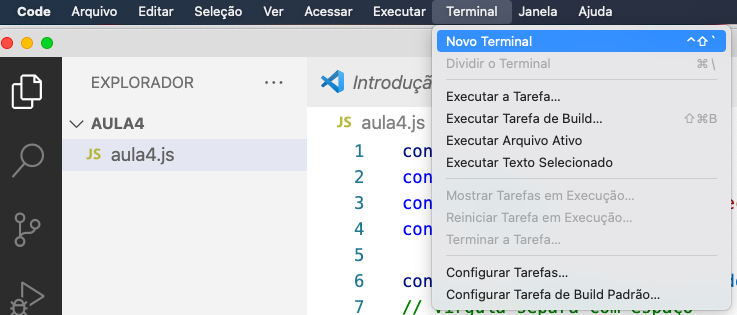
\includegraphics[width=80mm]{aulas/resources/aula_js_4_1.png}\\
            \tiny{ Acessando o terminal via VS Code \textbf{Fonte:} A autora.}
\end{frame}

%------------------------------------------------------------------------
\begin{frame}{Executar arquivos JS [2]}

    \begin{itemize}
        \item Ao acessar o terminal via VS Code, você não precisará navegar até o local do projeto, já estará nele.
        \item Digite \textcolor{red}{node arquivo.js}
        \item \textcolor{gray}{\textit{Você executou todo o arquivo js criado.}}
    \end{itemize}
    \centering
	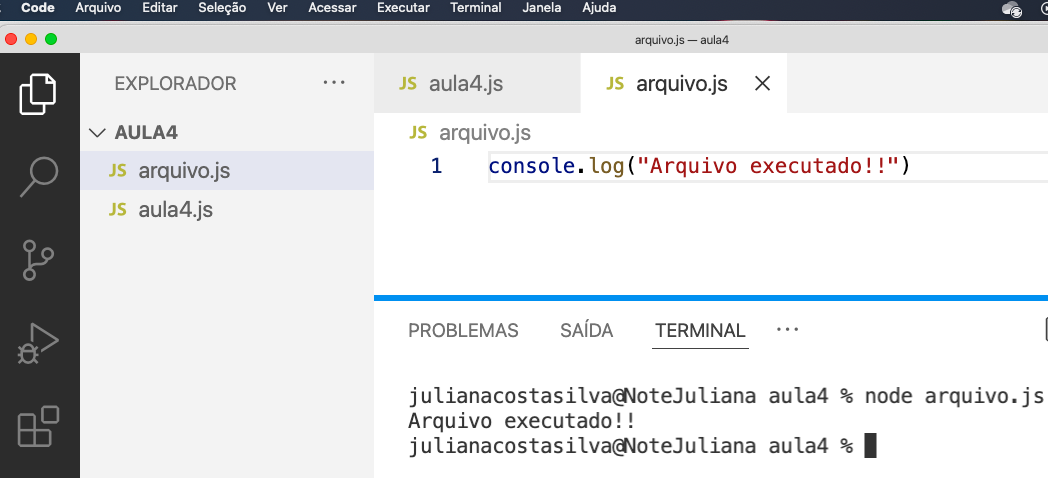
\includegraphics[width=80mm]{aulas/resources/aula_js_4_2.png}\\
            \tiny{ Executar arquivo js via terminal com VS Code \textbf{Fonte:} A autora.}
\end{frame}
%------------------------------------------------
\section{Tipos de variáveis}
\begin{frame}{Variáveis JS}
Teste o código abaixo:
    \centering
	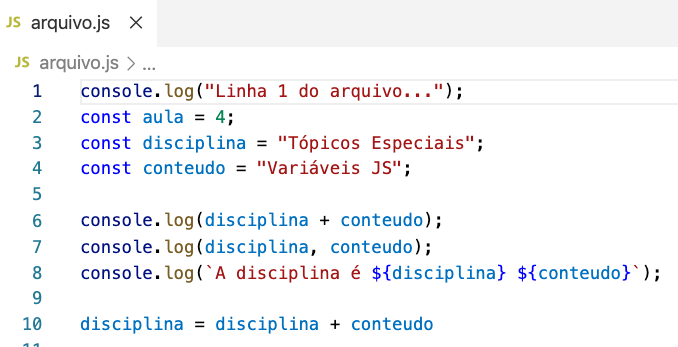
\includegraphics[width=80mm]{aulas/resources/aula_js_4_3.png}\\
    \tiny{ \textbf{Fonte:} A autora.}\\
    Execute arquivo.js via terminal pelo VS Code.
\end{frame}
%-----------------------------------------------------
    \begin{frame}{Resultado}
    \centering
	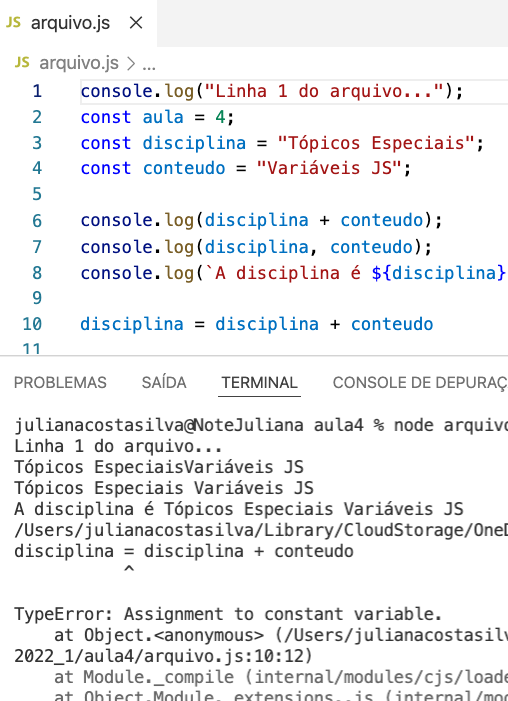
\includegraphics[width=50mm]{aulas/resources/aula_js_4_4.png}\\
            \tiny{\textbf{Fonte:} A autora}\\
            \textcolor{purple}{TypeError: Assignment to constant variable.}
    \end{frame}
%-----------------------------------------------------
    \begin{frame}{Declaração de variáveis JS}
    \begin{block}{O que é uma variável?}
    Uma variável é um container para um valor, como um número que podemos usar em uma operação de adição, ou uma sequência de texto que possamos usar como parte de uma oração. Mas uma coisa especial a respeito das variáveis é que seu conteúdo pode mudar.
    \end{block}
    \centering
    \vspace{0.5cm}
    \tiny{\textbf{Fonte:} \cite{moziladev2022js}}
    \end{frame}
    
%-----------------------------------------------------
    \begin{frame}{A diferença entre \textcolor{blue}{var} e \textcolor{blue}{let}}
    \begin{block}{var}
    Quando o JavaScript foi criado, havia apenas \textcolor{yellow}{var}. Isso funciona basicamente bem na maioria dos casos, mas tem alguns problemas na maneira como funciona, seu design pode ser confuso ou totalmente irritante.
    \end{block}
    
    \begin{block}{let}
    A declaração \textcolor{yellow}{let} foi criada nas versões modernas de JavaScript, uma nova palavra-chave para criar variáveis que funcionam de maneira um pouco diferente de \textcolor{yellow}{var}, corrigindo seus problemas no processo.
    \end{block}
    \centering
    %\vspace{0.5cm}
    \tiny{\textbf{Fonte:} \cite{moziladev2022js}}
    \end{frame}
    
    %-----------------------------------------------------
    \begin{frame}{A diferença entre \textcolor{blue}{var} e \textcolor{blue}{let} [2]}
    \begin{block}{var}
    \begin{itemize}
        \item A declaração \textcolor{yellow}{var} permite declarar uma variável depois que você a inicializa, isso resulta em código confuso e difícil de entender.
        \item Ao usar \textcolor{yellow}{var}, você pode declarar a mesma variável quantas vezes quiser. 
    \end{itemize}
    \end{block}
    
    \begin{block}{let}
    \begin{itemize}
        \item Com \textcolor{yellow}{let} você não consegue declarar uma variável depois que você a inicializa. 
        \item Com \textcolor{yellow}{let} você não consegue declarar uma variável varias vezes. 
        \item Com \textcolor{yellow}{let} é possível apenas atualizar o valor de uma variável, não declara-lá novamente.
    \end{itemize}
    \end{block}
    \centering
    %\vspace{0.5cm}
    \tiny{\textbf{Fonte:} \cite{moziladev2022js}}
    \end{frame}
    %TIPOS: 
    %Arrays - https://developer.mozilla.org/pt-BR/docs/Learn/JavaScript/First_steps/Variables
%-----------------------------------------------------
   \section{Atividade} 
   \begin{frame}{Atividade}
	??
	\begin{enumerate}
	    \item  ??
	\end{enumerate}
	
    \end{frame}
%------------------------------------------------------------------------
   \subsection{Referências}
    \begin{frame}{Referências}%[allowframebreaks]
\frametitle{Referências}
\small
\begin{center}
\tiny
\bibliographystyle{apalike}
\bibliography{ref_aula}
\end{center}
\end{frame}
\end{document}
